%%%% Pantalla(s) asociadas a caso de uso %%%%

\pagebreak
\hypertarget{IU1}{}
\section{IU1 Menú de Pizzas}

	%Descripción de la pantalla
	\noindent \textbf{Descripción de la pantalla}\\

		La pantalla mostrada en la figura \ref{IU1} tiene como objetivo permitir a los clientes mostrar el menú de pizzas que Pizza Planeta ofrece. 
		No se cuenta con campos de entrada. 
		
		El cliente podrá interactuar en la pantalla con los diferentes botones como se mostrará en la pantalla correspondiente a la figura \ref{IU1}.
		%Pantalla del sistema
		\begin{figure}[h]

			\begin{center}				

				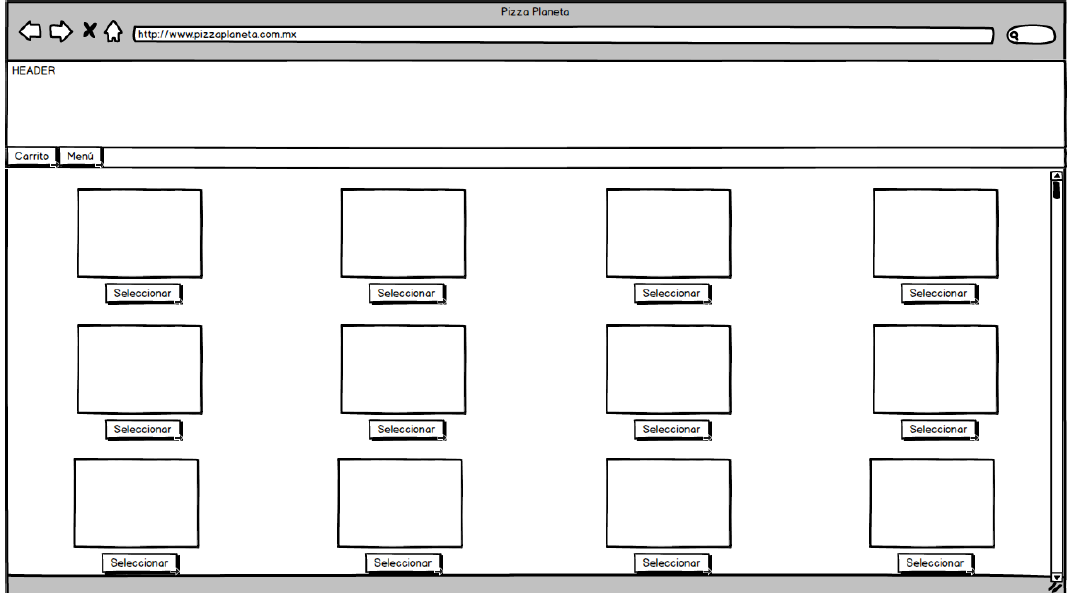
\includegraphics[scale=0.50]{./imagenes/IUs/RegistroSolicitantes/iu1-IniciarSesion/IU1-MenuDePizzas.png}
				\caption{IU1 Menú de Pizzas}
				\label{IU1}

			\end{center}
				
		\end{figure}


		El caso de uso \hyperlink{CU1}{CU1 Seleccionar Pizza}, describe de forma detallada el comportamiento asociado.

	%Acciones asociadas
	\noindent \textbf{\\Acciones en pantalla}

		\begin{itemize}

			\item 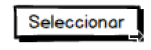
\includegraphics[scale=0.500]{imagenes/iconografia/Seleccionar.png}: Dirige a la pantalla \hyperlink{IU2}{IU2 Personaliza Pizza}
			\item 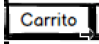
\includegraphics[scale=0.500]{imagenes/iconografia/Carrito.png}: Dirige a la pantalla \hyperlink{IU3}{IU3 Carrito de Compras}
			\item 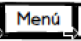
\includegraphics[scale=0.500]{imagenes/iconografia/Menu.png}: Dirige a la pantalla de la figura \ref{IU1}

		\end{itemize}
	
	\hypertarget{IU2}{}
	\section{IU2 Personaliza Pizza}
	
	%Descripción de la pantalla
	\noindent \textbf{Descripción de las pantallas}\\
	
	La pantalla mostrada en la figura \ref{IU2} tiene como objetivo permitir a los clientes seleccionar atributos referentes a la manera de preparación de la pizza seleccionada.
	Los campos de entrada son tamaño, tipo y cantidad, todos con la característica de ser obligatorios.
	
	El cliente podrá interactuar en la pantalla con los diferentes botones y listas como se mostrará en la pantalla correspondiente a la figura \ref{IU2}.
	%Pantalla del sistema
	\begin{figure}[h]
		
		\begin{center}				
			
			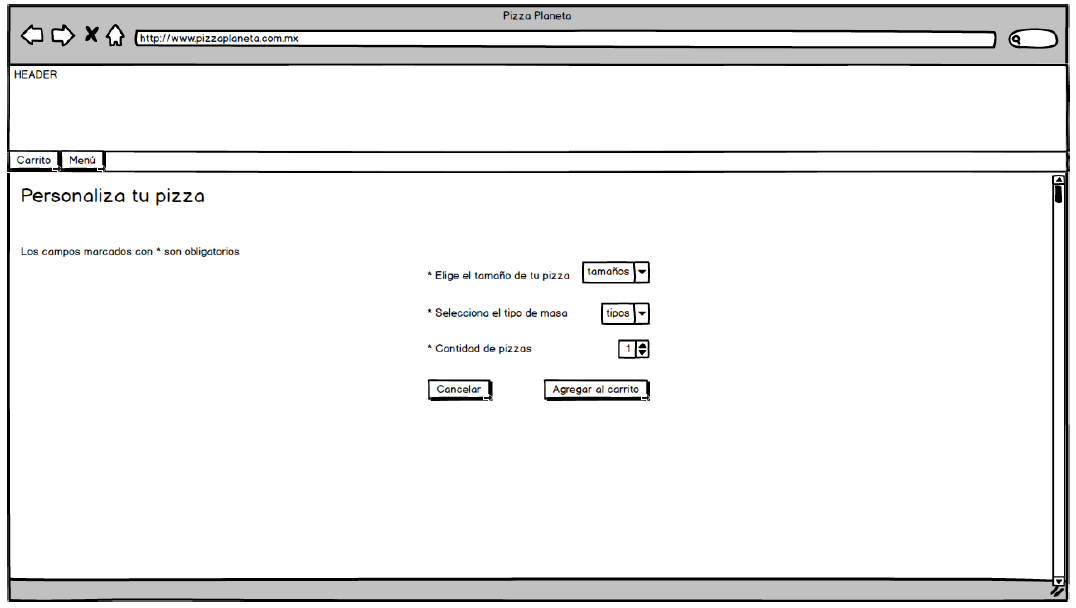
\includegraphics[scale=0.50]{./imagenes/IUs/RegistroSolicitantes/iu1-IniciarSesion/IU2-PersonalizaPizza.png}
			\caption{IU2 Personaliza Pizza}
			\label{IU2}
			
		\end{center}
		
	\end{figure}
	
	
	El caso de uso \hyperlink{CU1}{CU1 Seleccionar Pizza}, describe de forma detallada el comportamiento asociado.
	
	%Acciones asociadas
	\noindent \textbf{\\Acciones en pantalla}
	
	\begin{itemize}
		
		\item 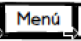
\includegraphics[scale=0.500]{imagenes/iconografia/Menu.png}: Dirige a la pantalla de la figura \ref{IU1}
		\item 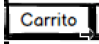
\includegraphics[scale=0.500]{imagenes/iconografia/Carrito.png}: Dirige a la pantalla de la figura \ref{IU3}
		\item 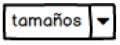
\includegraphics[scale=0.500]{imagenes/iconografia/Tamanos.png}: Permite seleccionar el tamaño deseado de la pizza.
		\item 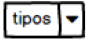
\includegraphics[scale=0.500]{imagenes/iconografia/Tipos.png}: Permite seleccionar la masa deseada para la pizza.
		\item 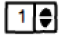
\includegraphics[scale=0.500]{imagenes/iconografia/Cantidad.png}: Permite seleccionar la cantidad de pizzas a agregar al carrito.
		\item 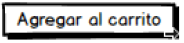
\includegraphics[scale=0.500]{imagenes/iconografia/AgregarCarrito.png}: Dirige a la pantalla de la figura \ref{IU2.1}
		\item 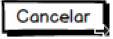
\includegraphics[scale=0.500]{imagenes/iconografia/Cancelar.png}: Dirige a la pantalla de la figura \ref{IU1}
		
		
		En la pantalla se mostrará un mensaje indicando que la orden fue agregada con éxito al carrito de compras.
		
		
			%Pantalla del sistema
		\begin{figure}[h]
			
			\begin{center}				
				
				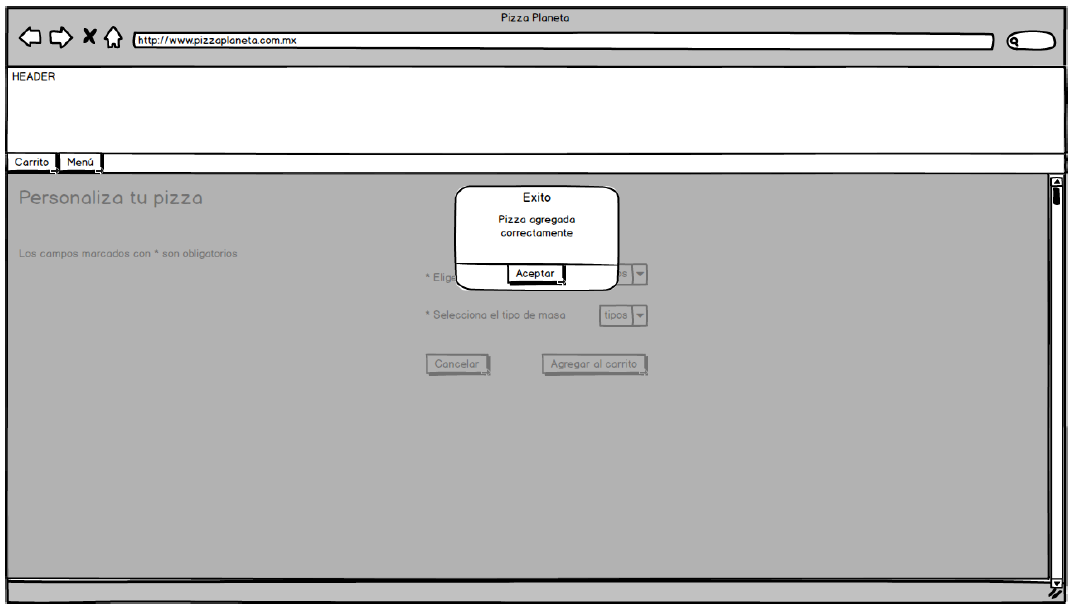
\includegraphics[scale=0.50]{imagenes/IUs/RegistroSolicitantes/iu1-IniciarSesion/IU2-1-PersonalizaPizzaMensaje.png}
				\caption{IU2.1 Personaliza Pizza Mensaje}
				\label{IU2.1}
				
			\end{center}
			
		\end{figure}
	
	\noindent \textbf{\\Acciones en pantalla}
	
		\begin{itemize}
		
		\item 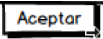
\includegraphics[scale=0.500]{imagenes/iconografia/Aceptar.png}: Dirige a la pantalla de la figura \ref{IU1}
		
	\end{itemize}
		
	\end{itemize}

\hypertarget{IU3}{}
\section{IU3 Carrito de Compras}

%Descripción de la pantalla
\noindent \textbf{Descripción de las pantallas}\\

La pantalla mostrada en la figura \ref{IU3} tiene como objetivo mostrar a los clientes las compras que han sido agregadas al carrito de compras.
No se cuenta con campos de entrada.

El cliente podrá interactuar en la pantalla con los diferentes botones como se mostrará en la pantalla correspondiente a la figura \ref{IU3}.
%Pantalla del sistema
\begin{figure}[h]
	
	\begin{center}				
		
		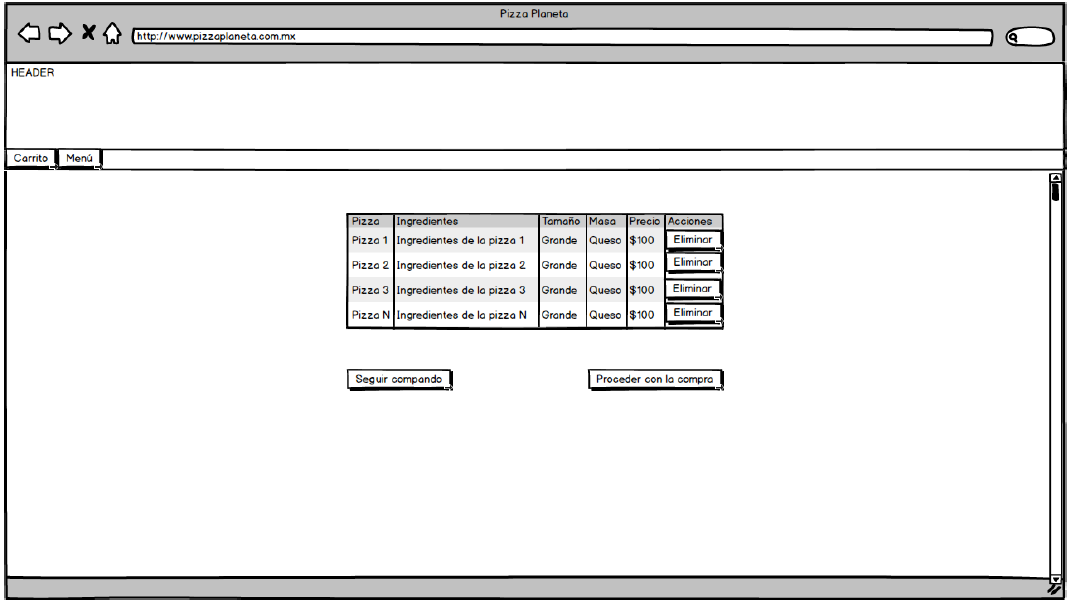
\includegraphics[scale=0.50]{./imagenes/IUs/RegistroSolicitantes/iu1-IniciarSesion/IU3-CarritoDeCompras.png}
		\caption{IU3 Carrito de Compras}
		\label{IU3}
		
	\end{center}
	
\end{figure}


El caso de uso \hyperlink{CU2}{CU2 Ver Carrito de Compras}, describe de forma detallada el comportamiento asociado.

%Acciones asociadas
\noindent \textbf{\\Acciones en pantalla}

\begin{itemize}
	
	\item 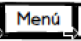
\includegraphics[scale=0.500]{imagenes/iconografia/Menu.png}: Dirige a la pantalla de la figura \ref{IU1}
	\item 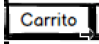
\includegraphics[scale=0.500]{imagenes/iconografia/Carrito.png}: Dirige a la pantalla de la figura \ref{IU3}
	\item 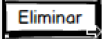
\includegraphics[scale=0.500]{imagenes/iconografia/Eliminar.png}: Permite eliminar alguna de las opciones agregadas con anterioridad al carrito.
	\item 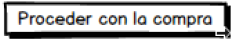
\includegraphics[scale=0.500]{imagenes/iconografia/Proceder.png}: Dirige a la pantalla de la figura \ref{IU4}
	
	En la pantalla se mostrará un mensaje indicando que si se está seguro de querer eliminar esa pizza.
	
	
	%Pantalla del sistema
	\begin{figure}[h]
		
		\begin{center}				
			
			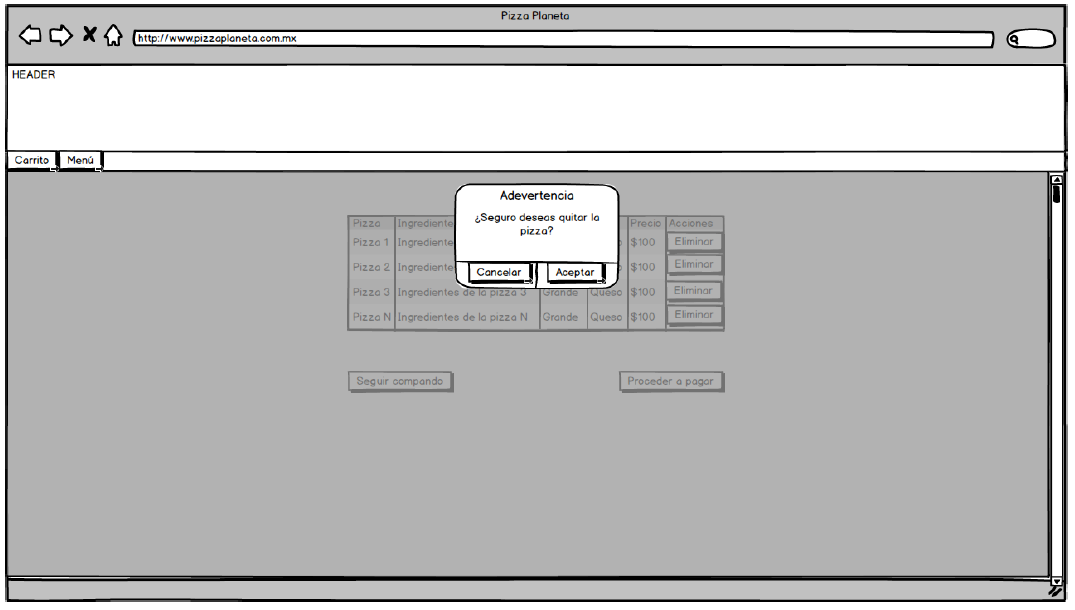
\includegraphics[scale=0.50]{imagenes/IUs/RegistroSolicitantes/iu1-IniciarSesion/IU3-1CarritoDeComprasQuitar.png}
			\caption{IU3.1 Carrito de Compras Quitar}
			\label{IU3.1}
			
		\end{center}
		
	\end{figure}
	
	\noindent \textbf{\\Acciones en pantalla}
	
	\begin{itemize}
		
		\item 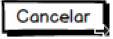
\includegraphics[scale=0.500]{imagenes/iconografia/Cancelar.png}: Dirige a la pantalla de la figura \ref{IU3}
		\item 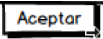
\includegraphics[scale=0.500]{imagenes/iconografia/Aceptar.png}: Dirige a la pantalla de la figura \ref{IU3.2}
		
	\end{itemize}

	%Pantalla del sistema
\begin{figure}[h]
	
	\begin{center}				
		
		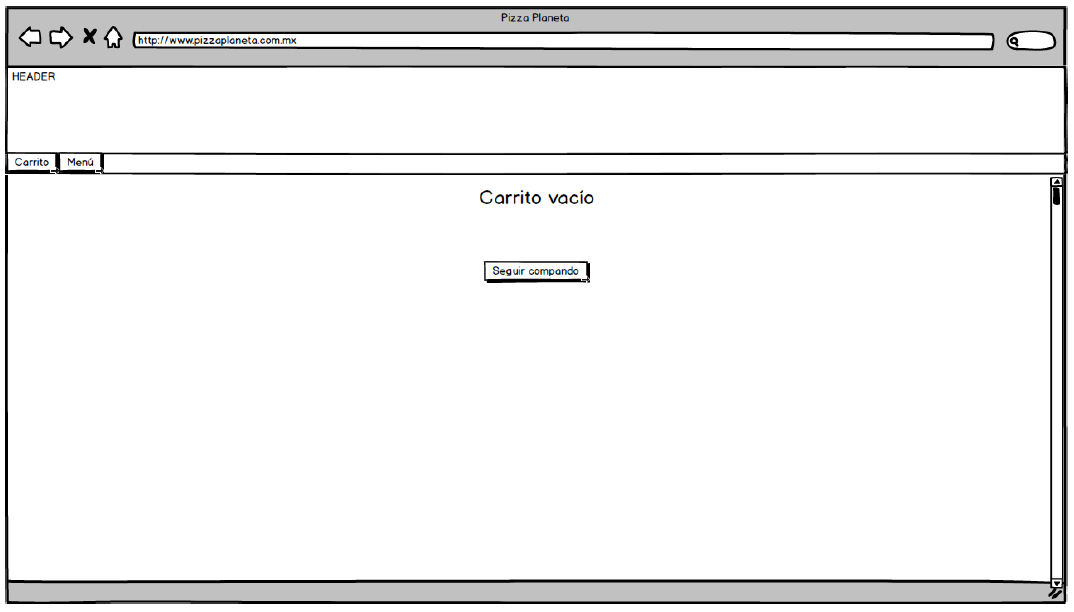
\includegraphics[scale=0.50]{imagenes/IUs/RegistroSolicitantes/iu1-IniciarSesion/IU3-2CarritoDeComprasVacio.png}
		\caption{IU3.2 Carrito de Compras Vacío}
		\label{IU3.2}
		
	\end{center}
	
\end{figure}
	
\noindent \textbf{\\Acciones en pantalla}
	
	\begin{itemize}
		
		\item 
\includegraphics[scale=0.500]{imagenes/iconografia/Seguir.png}: Dirige a la pantalla de la figura \ref{IU1}
		
	\end{itemize}

\end{itemize}

\hypertarget{IU1}{}
\section{IU4 Datos de Compra}

%Descripción de la pantalla
\noindent \textbf{Descripción de la pantalla}\\

La pantalla mostrada en la figura \ref{IU4} tiene como objetivo permitir a los clientes ingresar sus datos para poder continuar con su compra.
Los campos de entrada son datos necesarios para poder lograr el envío exitosamente (nombre, teléfono, correo, calle, número, cp, colonia, delegación, estado, tipo de envío) y están marcados como obligatorios.

El cliente podrá interactuar en la pantalla con los diferentes botones y  como se mostrará en la pantalla correspondiente a la figura \ref{IU4}.
%Pantalla del sistema
\begin{figure}[h]
	
	\begin{center}				
		
		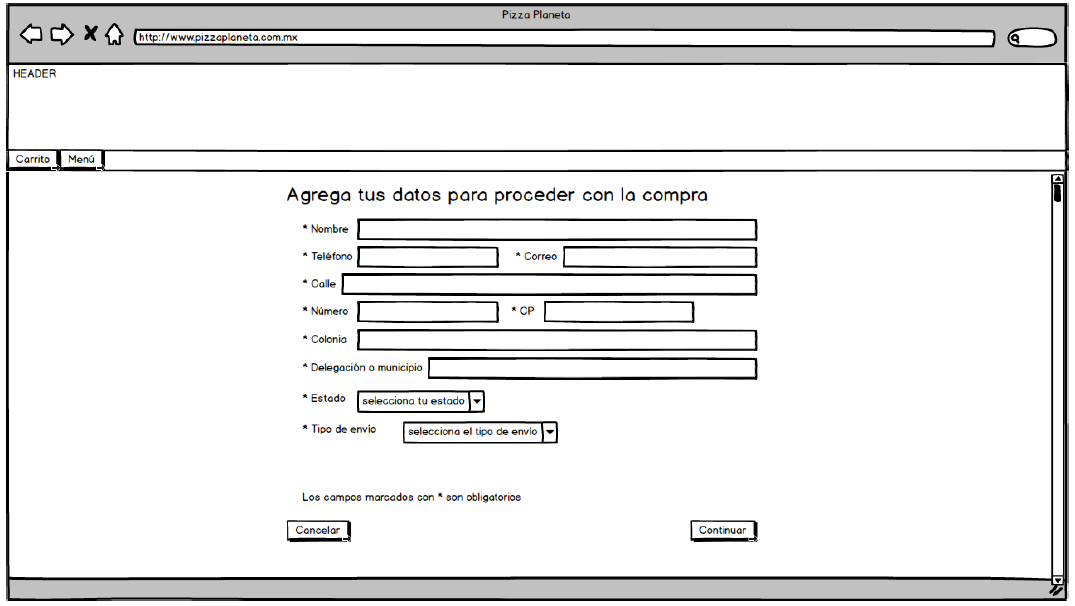
\includegraphics[scale=0.50]{./imagenes/IUs/RegistroSolicitantes/iu1-IniciarSesion/IU4-DatosDeCompra.png}
		\caption{IU4 Datos de Compra}
		\label{IU4}
		
	\end{center}
	
\end{figure}


%El caso de uso \hyperlink{CU3}{CU3 Relizar Compra de Pizza}, describe de forma detallada el comportamiento asociado.

%Acciones asociadas
\noindent \textbf{\\Acciones en pantalla}

\begin{itemize}
	
	\item \textbf{Nombre:} Permite ingresar el nombre del cliente.
	\item 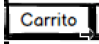
\includegraphics[scale=0.500]{imagenes/iconografia/Carrito.png}: Dirige a la pantalla \hyperlink{IU3}{IU3 Carrito de Compras}
	\item 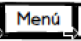
\includegraphics[scale=0.500]{imagenes/iconografia/Menu.png}: Dirige a la pantalla de la figura \ref{IU1}
	
\end{itemize}

